\documentclass[../../thesis.tex]{subfiles}
\graphicspath{{\subfix{diagrams/}}}

\begin{document}
When being launched in 2015, Ethereum \cite{wood2014ethereum} set out to change the way we compute. A trustless, permissionless, and decentralized world computer was envisioned, set to open a new class of applications. The importance of running verifiable, Turing-complete code in a permissionless and trustless manner cannot be overstated and enables products and services not thought to be possible. However, the technical limitations have also become apparent quickly. Computations are expensive, theoretical transactions per second are low, and the overall throughput has been stagnant. While Eth2 gives a path towards scaling the network, it is expected to take years to complete. 

The first major use case for Ethereum was tokenization. With the development of the ERC-20 standard, launching a token on the Ethereum blockchain was trivial. As tokens run as smart-contracts on the Ethereum blockchain, they are secured by its proof of work consensus, which, given Ethereums PoW hash rate, makes consensus attacks infeasible. Running on Ethereum blockchain is a significant benefit when looking to tokenize things, as network security can be assumed. While tokenizations are a step in the right direction, they do not come close to the initial vision. While the standardization enables simple integrations into exchanges and wallets, most tokens are isolated in their functionality and ecosystem and lack productive usage.
\todo{token all isolated, not working together... Not a lot of gas needed blabla}

With all of these developments over the past couple of years, it seems we have now entered a new phase of smart-contract use-cases, namely Decentralized Finance (DeFi). While DeFi has many different products and functionalities, at its core aims to utilize tokenized assets in some productive form. 


Lending and collateralized borrowing is possible with Aave \cite{kulechov_2020}, assets can be deposited into liquidity pools\cite{adams2020uniswap} to generate yields, flash-loans \cite{kulechov_2020}\cite{adams2020uniswap} enabled uncollateralized borrowing as long as the loan is repaid in the same transaction and assets can be traded in a non-custodial way with Uniswap \cite{adams2020uniswap} \todo{Mention other swap protocols?}. It can be questioned how useful or necessary these protocols really are, but the core idea behind them is impressive. Rebuilding traditional financial products, running as non-custodial and permission-less smart-contracts, all based on the same standardizations, has the potential to reshape the way finance works. With these developments not looking to slow down, they are quickly overwhelming the Ethereum blockchain, pushing transaction costs \cite{gasprice} higher and higher. 

One of these new DeFi applications is Uniswap \cite{adams2020uniswap}. Uniswap is a crypto-asset exchange running as a collection of smart-contracts on the Ethereum blockchain, enabling non-custodial, trust-less, and permission-less trading of ERC-20 assets. Since its running on the Ethereum Blockchain, reducing the computational complexity of trade execution is essential for making it a viable product. In typical crypto-asset exchanges, trading is built around a central order book. Users can add buy or sell orders for a given trading pair, and a matching engine checks if these orders can be matched, executing the trade once they do. While running this on modern server infrastructure is feasible, running it on the blockchain is not. The demand for memory and processing power is too large, so a different approach must be taken. Uniswap solves this by applying the automated market maker (AMM) model, which will be explained in detail in sec. XX. By applying this model, Uniswap reduces the computational complexity to make this a viable business model. At least it was, when Uniswap launched. 

\begin{figure}[h]
    \centerline{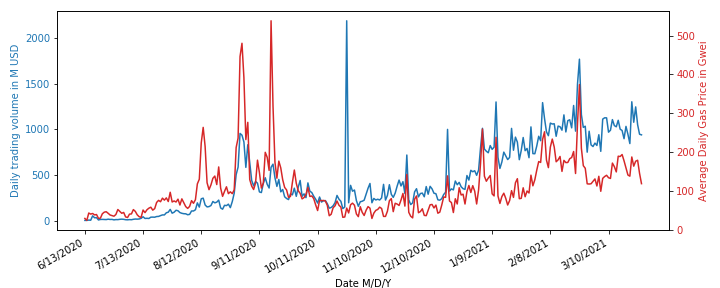
\includegraphics[totalheight=5.6cm]{diagrams/gas_volume.png}}
    \caption{Combined daily Uniswap trading volume in million USD and average daily Ethereum gas price}
    \label{fig:gas_vol}
\end{figure}

The recent rise of Ethereums gas price \cite{gasprice} can also be attributed to the growing popularity of Uniswap. Currently, it is one of the most used smart-contract on the Ethereum blockchain, making up on average around 15\% of gas \cite{eth_gas_guzzlers} usage of a block at the time of writing. To date, it accrued over \$280 million in transaction fees \cite{uniswap_tx_fees} and has settled over \$100 billion in trading volume \cite{cummulative_vol}. With the gas price having reached 500 gwei on a couple of occasions, a single Uniswap trade can cost upwards of \$130. While it would be assumed that high gas prices cause a reduction in trading volume, the opposite is the case. As shown in F.\ref{fig:gas_vol} there seems to be a strong correlation between daily trading volume on Uniswap and the average daily Ethereum gas price, so reducing gas consumption by Uniswap transactions should result in a reduced gas price for the entire network.

With longer-term scaling solutions in development but still years away, a shorter-term solution is needed. A couple of short-term scaling approaches have been proposed. While these do differ, they all aim to move transactional data to a layer-2\footnote{A layer-2 system is a data storage that does not reside on the blockchain but has its state committed to it in some way} system, while ensuring correctness of that data in some way. One of the approaches is called zk-rollup, the focus of this work. Moving data to a layer-2 system can increase the number of transactions that fit into a block while also reducing transaction costs for the user, with is beneficial for Uniswap users and all other participants of the Ethereum network. 

Current zk-rollup enabled applications running on the Ethereum mainnet, one of them being ZK Sync, are focused on reducing cost of Ether and ERC-20 transfers\todo{not a great sentence}. Users deposit funds into its smart-contract, which results in the user's deposit being represented as balance in layer-2. When a user makes a transfer to another user, the involved balances get updated in layer-2, while the correctness of these updates is ensured via zkSNARK. It is important to note, that ZK Sync acts as a closed system, transfers only change balances in layer-2, while deposited funds in the smart-contract do not move. While this approach has significantly reduced costs of transfers, it only marks the first generation of potential(?) zk-rollup enabled apps.

Aggregating Uniswap trades is an interesting application to explore the potential of zk-rollup technology. It combines the layer-2 storing and updating of balances already done by ZK Sync while opening the system to interact with other smart-contracts. When aggregating trades, we need to interact with the Uniswap contracts to execute the aggregated trade, then update the layer-2 balances according to the trade and verify everything via zkSNARK. It is the next step in exploring the potential of zk-rollups as a generalizable scaling solution, applicable to any kind of smart-contract. 

\end{document}